% Section content template for individual Educative lessons
% This file contains the actual content for a specific section
% Generated from Educative API section content

% Section: Getting Ready: The Airline Management System
% Section ID: 5983485107109888
% Section Slug: getting-ready-the-airline-management-system
% Generated: 2025-12-14T13:16:34.908148

\subsection{Problem definition}\label{3qde8BUUnW7vlI44PkzKp}
\\
An \textbf{airline management system} is a software used to efficiently manage all activities within an airline's system. Nowadays, every airline has a management system to digitize the process of scheduling flights, managing staff, ticket reservations, and performing other necessary airline management tasks. Moreover, the system tracks the number of aircraft, pilots, and their availability at airports. The system provides customers the complete flight information to view the available flights and schedule them online. The front desk officer should be able to reserve tickets, create itineraries, and process flight payments for customers, providing a smoother booking experience for those who prefer or require in-person assistance. Similarly, the admin can manage all the airline activities with the help of this system. Therefore, the airline management system facilitates its customers and administrators, controlling all operations of the airline company.

\begin{figure}[htbp]
 \centering
 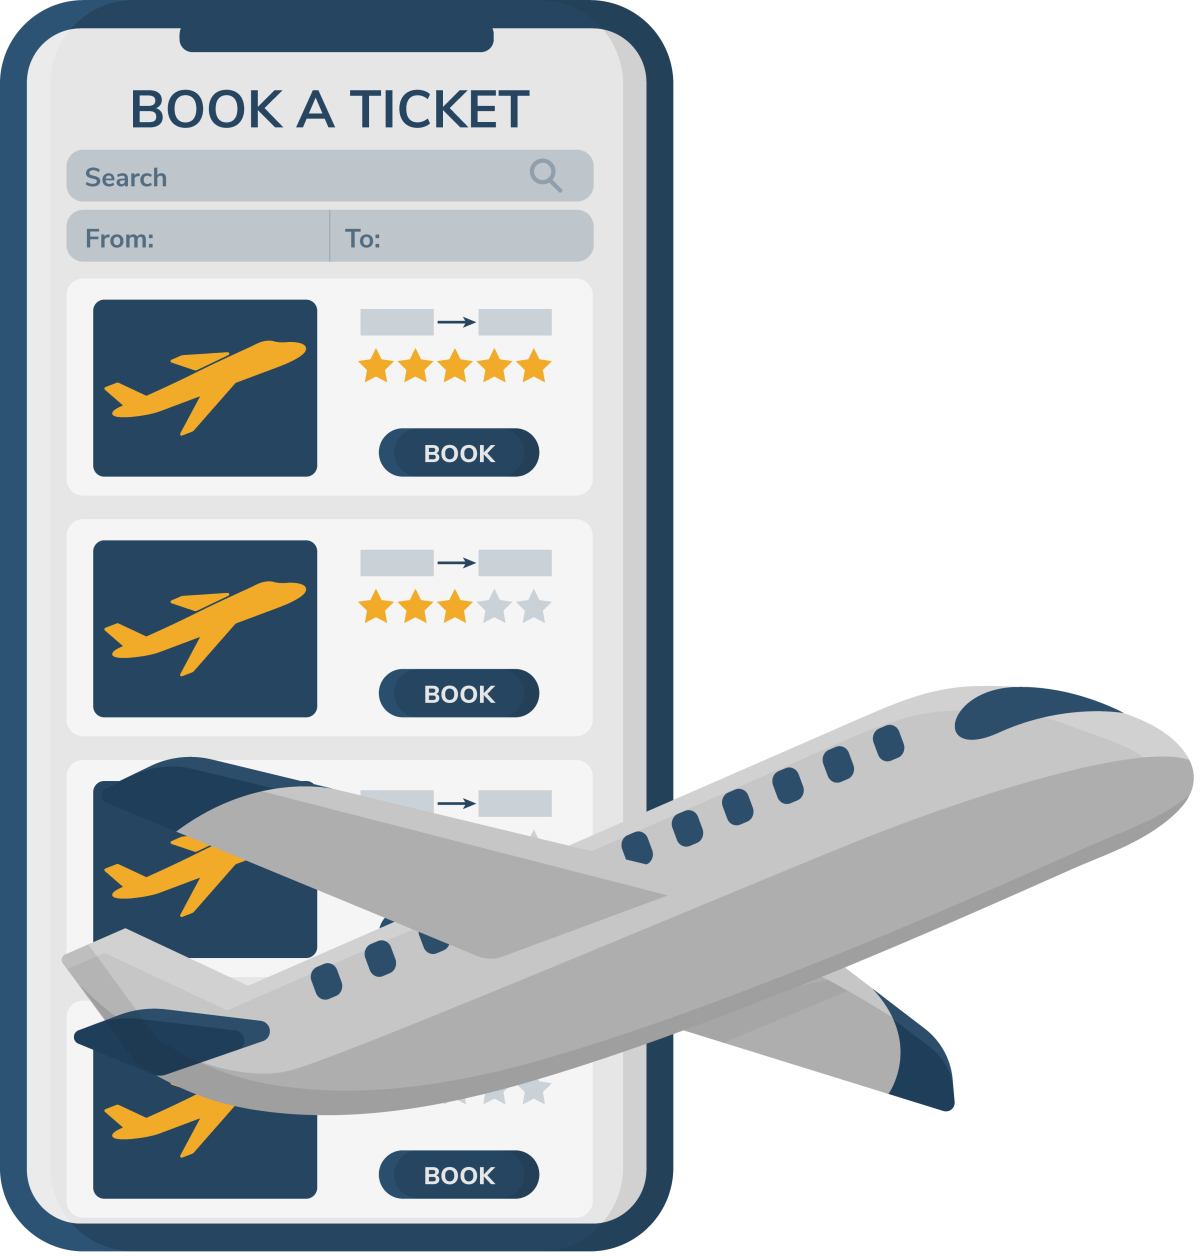
\includegraphics[width=0.15\textwidth]{Images/chapter_25/section_5983485107109888/6505597303521280.png}
 \caption{Airline management system}
\end{figure}

\subsection{Expectations from the interviewee}\label{wkVURSXPJBofYespagGFE}
\\
The airline management system comprises several components, each with its own specific constraints and requirements. The following provides an overview of some of the main things that the interviewer will want to hear you discuss in more detail during the interview.

\subsubsection{Flight reservation}\label{G7woD7WtXV9EPxz16RdLF}
\\
Flight reservation is a crucial component of an airline's management system. The system must ensure that no two people are assigned to the same seat. The interviewer expects you to ask questions to identify how the system will complete flight reservations:

\begin{itemize}
\item
\protect\phantomsection\label{-eWR0r5OXnO2_b0IYztPA}
How will the system ensure that multiple users do not have the same seat on the aircraft?
\item
\protect\phantomsection\label{p6SR5O-WTMEn5sybQ3IiU}
Can one itinerary reserve multiple flights?
\item
\protect\phantomsection\label{4XUP_bA4QywxZo9OzyfsF}
Can the customer reserve the whole aircraft?
\end{itemize}

\subsubsection{Payment handling}\label{oCIUzeNtqXnruNjQEMTG6}
\\
One of the airline management system's most significant attributes is its payment structure for its customers. This can vary, so the interviewer would expect you to ask the questions listed below:

\begin{itemize}
\item
What payment methods are accepted, such as credit cards or cash?
\item
How does the customer make the payment? Does the customer pay online or in person?
\item
Will the customer be able to pay in advance for a flight booking, or is a just-in-time (JIT) payment method available?
\end{itemize}

\subsubsection{Price variance}\label{vF2EnW1Q6tClFed2Waw4G}
\\
Now that we've discussed the payment methods of the airline management system, let's ask the interviewer about the pricing model. You may ask the questions listed below:

\begin{itemize}
\item
Is the price set manually, or does the system calculate the price for each flight?
\item
Do all seats have the same price, or is it calculated based on the seat type?
\item
Do weekdays and weekends affect the price of the flight?
\item
Is the price of the flight affected by an increase in demand?
\item
How does the duration of the flight affect the payment?
\end{itemize}

\subsubsection{Flight cancellation}\label{-zL_WWOLPzBEZtlfVs172}
\\
In the airline management system, customers may want to cancel a flight after booking it. Therefore, you can ask the following questions:

\begin{itemize}
\item
\protect\phantomsection\label{M0daI0KAMljqeZRkZWL-v}
Can the customer cancel a flight?
\item
\protect\phantomsection\label{okI6-u03zPazrAcR0KC7u}
What is the time limit to cancel the flight?
\item
\protect\phantomsection\label{PfSrKQ0T0PGC3Q6cd86LY}
Which type of users are allowed to request a flight cancellation?
\end{itemize}

\subsubsection{Flight scheduling}\label{zHDdi0HPuBmiiKtD25-OQ}
\\
Flight scheduling is crucial for ensuring timely and conflict-free operations. The interviewer might expect you to ask:

\begin{itemize}
\item
\protect\phantomsection\label{FxlmLlbRg0HsJ9khpFAP2}
How is a flight schedule created and managed?
\item
\protect\phantomsection\label{PT3D7PZ3EGW2pXGyKBAKU}
Can a flight be delayed or rescheduled, and how is this handled in the system?
\item
\protect\phantomsection\label{2WgpY1kwWcmGWcVq1-TeH}
Is there any buffer time considered between flights for aircraft and crew?
\end{itemize}

\subsubsection{Staff and crew management}\label{XUj2h4Yw1hNSz7fd7BOR5}
\\
Managing pilots and crew availability is vital for operations. You may want to ask:

\begin{itemize}
\item
\protect\phantomsection\label{OqcKHlhV_84gU5XqVOar9}
How is crew availability tracked in the system?
\item
\protect\phantomsection\label{HunjEM3ageULf71s9J8yR}
Can crew members be assigned to multiple flights in a day?
\item
\protect\phantomsection\label{mje0pZhjgUk3f1N-CmYge}
What happens if a crew member becomes unavailable suddenly?
\end{itemize}

\subsection{Design approach}\label{nf4nt6YzKOQV2im_KzbAe}
\\
We'll design this airline management system using the bottom-up approach. For this purpose, we will follow the steps below:

\begin{itemize}
\item
Identify and design the smallest components first, including the seat, flight, etc.
\item
Use these small components to design larger components, such as an airport or an aircraft that can be composed of multiple seats.
\item
\protect\phantomsection\label{5wKV0fxaBgn54tRtFwdan}
Repeat the steps above until the entire airline management system is designed.
\end{itemize}

\subsection{Design pattern~}\label{RkUk9f5tCVw9Mt0XSGqOi}
\\
During an interview, it is always a good practice to discuss the design patterns that an airline management system falls under. Stating the design patterns gives the interviewer a positive impression and shows that the interviewee is well-versed in the advanced concepts of object-oriented design.
\\
Try to answer the following question. If you are not familiar with design patterns, don't worry! You can learn about them by asking, ``Define design patterns.''

\textbf{Question:}

Which design pattern(s) should be used to design an airline management system? Please elaborate on your choice(s).

Let's explore the requirements of the airline management system in the next lesson.

\subsection{}\label{bkBnriBdAM2Y-JRWZ9S2F}

% End of section content